\chapter{Experimental Results and Discussion}
\label{Chapter5}

\section{Results}

\textit{[TODO: Once additional candidates from Chapter~\ref{Chapter4} are
implemented, report a final cross-candidate comparison table here using the
metrics defined in Section~\ref{sec:metrics}.]}

The results below are an internal ablation of the LAMD-based candidate
only (baseline reimplementation vs.\ its own optimized versions,
Section~\ref{sec:lamd-candidate}), not yet a comparison against other
candidate methods. They were reconstructed from development logs and prior
analysis sessions rather than freshly re-run for this write-up; the exact
figures should be treated as best-available and re-verified before being
cited as final thesis results.

Table~\ref{tab:cache-ablation} isolates the effect of the semantic cache
alone, on a single 24-CFG APK, comparing no cache against a cold cache
(empty at the start of the run) and a warm cache (already populated by a
prior run on similar code). All three configurations agree on the
MALWARE verdict.

Neither configuration was billed per token: the LAMD-based candidate's
backend is accessed through a CLI-driven subprocess under a flat-rate
account rather than a directly billed API (Section~\ref{sec:lamd-candidate}),
so no invoice-level dollar figure exists for these runs. The \emph{estimated}
cost rows below apply the backend model's public list price as of this
writing (\$5 per million input tokens, \$30 per million output tokens) to
the token counts already reported, using the input/output split observed
directly in this candidate's own logged runs ($\approx$70\% input,
$\approx$30\% output) where a per-call split was not separately recorded.
These figures answer "what would this have cost under standard API
billing", not "what was actually paid" -- they are included because
Chapter~\ref{Chapter3}'s RQ2 (Section~\ref{sec:rq2}) treats a per-APK dollar
figure as central to comparing LLM-based detectors, and omitting one
entirely would leave that comparison axis unaddressed for this candidate.

\begin{table}[ht]
\centering
\caption{Effect of the semantic cache on the same 24-CFG APK}
\label{tab:cache-ablation}
\begin{tabular}{@{}lrrr@{}}
\toprule
 & No cache & Cold cache & Warm cache \\
\midrule
LLM calls        & 62      & 30 ($-52\%$)  & \textbf{9 ($-85\%$)} \\
Total tokens      & 146{,}533 & 78{,}749 ($-46\%$) & \textbf{41{,}598 ($-72\%$)} \\
Cache hit rate    & --      & 14/24         & \textbf{24/24} \\
Est.\ cost (USD)$^*$ & \$1.83 & \$0.98 ($-46\%$) & \textbf{\$0.52 ($-72\%$)} \\
Prediction        & MALWARE & MALWARE       & MALWARE \\
\bottomrule
\end{tabular}
\vspace{2pt}
\footnotesize\textit{$^*$Estimated at \$5/1M input + \$30/1M output tokens
(backend list price at time of writing) applied to this run's total token
count via the $\approx$70/30 input/output split observed elsewhere in this
candidate's logs -- not an actual per-token invoice; see text above.}
\end{table}

Table~\ref{tab:paired-comparison} reports a paired baseline-vs-improved
comparison on 6 fresh AndroZoo malware APKs, run once each through the
unoptimized baseline and the current cache-and-verified-connection design.
One case (\texttt{032EF910\ldots}) is excluded from the reduction column: at
the time of this run it exposed the missing-sink-API gap described in
Section~\ref{sec:lamd-candidate}, so the two pipelines used the same evidence
and reached different verdicts by chance rather than by design; after that
fix, the improved pipeline recovers the correct verdict.

\begin{table}[ht]
\centering
\caption{Paired baseline-vs-improved comparison, 6 malware APKs}
\label{tab:paired-comparison}
\begin{tabular}{@{}lrrrl@{}}
\toprule
APK & Baseline calls & Improved calls & Reduction & Prediction \\
\midrule
008C3C11\ldots & 124 & 54 & 56\% & MALWARE (both) \\
019B34A0\ldots & 97  & 48 & 51\% & MALWARE (both) \\
04C5329F\ldots  & 91  & 28 & 69\% & MALWARE (both) \\
05B7569D\ldots  & 89  & 3  & 97\% & MALWARE (both, post-fix) \\
\bottomrule
\end{tabular}
\end{table}

Across the full 12-APK set (7 malware, 5 benign), the improved pipeline
reached the correct verdict on 11/12 samples (91.7\%, rounded to 92\%
elsewhere in this chapter) after both design fixes described in
Section~\ref{sec:lamd-candidate}, up from 10/12 (83\%) before those fixes.
The one remaining miss was traced to Tier-3's verdict not being fully
deterministic across repeated LLM calls on the same borderline evidence,
rather than to either fixed design issue -- noted here as an open point,
discussed further in Section~\ref{sec:threats-ch5}. The miss is itself a
malware sample misclassified as benign (a false negative); the other 6
malware and all 5 benign samples are correct, giving
$\mathrm{TP}=6,\mathrm{FN}=1,\mathrm{TN}=5,\mathrm{FP}=0$, i.e.\ Precision
$=100\%$ and Recall $=85.7\%$ -- the figures quoted in
Section~\ref{sec:threats-ch5}.

\section{Discussion}

\textit{[TODO: Interpret the results. Compare against the related work
reviewed in Chapter~\ref{Chapter2}. Explain any surprising findings, and
directly answer the research questions stated in Chapter~\ref{Chapter1}.]}

\section{Threats to Validity}\label{sec:threats-ch5}

\subsection{Dataset Size and Selection Bias (Primary Threat)}

The 92\% figure above, like every other result in this chapter, is measured
on the 12-APK development set described in Section~\ref{sec:lamd-candidate}:
a small sample hand-curated at extreme VirusTotal confidence
($\texttt{vt\_detection}\geq15$ malware, $\texttt{vt\_detection}=0$ benign)
and balanced 7:5 malware-to-benign. This is the single most consequential
threat to the results in this chapter, and it is not merely a theoretical
concern -- it is directly measurable within this project. A separate,
unfiltered random sample of 750 AndroZoo APKs (no confidence threshold, no
class balancing, i.e.\ a realistic deployment-like distribution) is being
run through the same candidate design on two different self-hosted LLM
backends (``fit'', a locally hosted Qwen3.6-27B, and ``iec'', a second
self-hosted model) -- an in-progress run, 596/750 and 215/750 complete
respectively at time of writing, and the \texttt{fit} figures additionally
mix results from before and after a mid-run dataset rebalance (see caption).
Figure~\ref{fig:dataset-bias} reports accuracy, precision, and recall on
all three.

\begin{figure}[htbp]
\centering
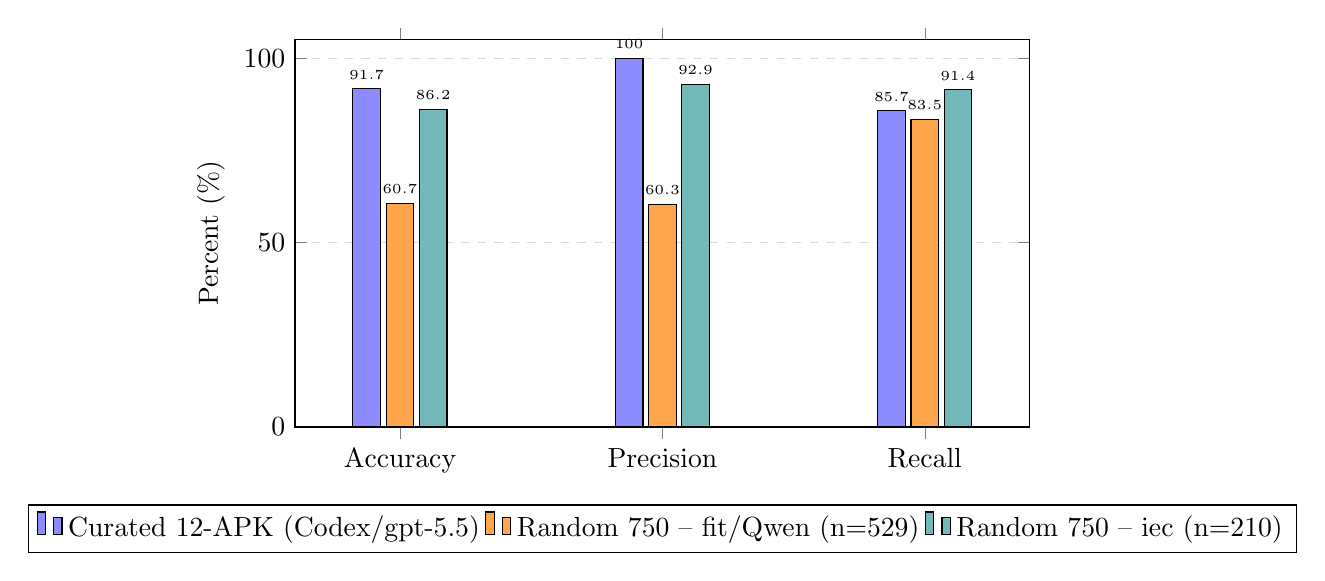
\begin{tikzpicture}
\begin{axis}[
    ybar,
    bar width=10pt,
    width=0.9\textwidth,
    height=6.5cm,
    ymin=0, ymax=105,
    ylabel={Percent (\%)},
    symbolic x coords={Accuracy, Precision, Recall},
    xtick=data,
    enlarge x limits=0.2,
    legend style={at={(0.5,-0.2)}, anchor=north, legend columns=-1},
    nodes near coords,
    nodes near coords align={vertical},
    every node near coord/.append style={font=\tiny},
    ymajorgrids=true,
    grid style={dashed, gray!30},
]
\addplot[fill=blue!45] coordinates {(Accuracy,91.7) (Precision,100) (Recall,85.7)};
\addplot[fill=orange!70] coordinates {(Accuracy,60.7) (Precision,60.3) (Recall,83.5)};
\addplot[fill=teal!55] coordinates {(Accuracy,86.2) (Precision,92.9) (Recall,91.4)};
\legend{Curated 12-APK (Codex/gpt-5.5), Random 750 -- fit/Qwen (n=529), Random 750 -- iec (n=210)}
\end{axis}
\end{tikzpicture}
\caption{Detection performance on the curated 12-APK development set versus
an in-progress, unfiltered random sample of 750 AndroZoo APKs run on two
different backends. Figures for the random sample reflect partial progress
at the time of writing (596/750 fit, 215/750 iec) and will change as the
run completes; the \texttt{fit} column additionally mixes results from
before and after a mid-run dataset rebalance (25\% of the 750 pool was
swapped to reach a 50:50 malware:benign split partway through), so it
should be read as directional, not final. Recomputed via
\texttt{results/compute\_accuracy.py} against ground truth reconstructed
from the original AndroZoo VirusTotal metadata.}
\label{fig:dataset-bias}
\end{figure}

Recall holds up across all three (83.5--91.4\%), so the pipeline is not
missing more real malware on the unfiltered sample. Precision, however,
diverges sharply by \emph{backend}: on \texttt{iec} it stays close to the
curated set (92.9\% vs.\ 100\%), while on \texttt{fit} it collapses to
60.3\%. Since the curated 12-APK figures were themselves produced on a
third backend (Codex CLI/gpt-5.5, Section~\ref{sec:lamd-candidate}), this
comparison cannot cleanly separate a ``dataset difficulty'' effect from a
``backend'' effect -- both vary at once between the curated and random
runs, and the \texttt{fit} vs.\ \texttt{iec} gap on the \emph{same}
unfiltered sample shows the backend effect alone is already large. What
can be said without that confound: the pipeline's false-positive behavior
is not a fixed property of the design, and evaluating it on one
easy, class-balanced, high-confidence, single-backend sample --
as the 92\% headline figure in this chapter does -- is not sufficient to
characterize it. Root-caused false positives on the \texttt{fit} run trace
to legitimate-but-suspicious-looking patterns (e.g.\ login flows that read
credential fields before a network call, or reflection-based library
internals such as OkHttp's certificate-chain cleaner) that the curated
set's hand-picked samples do not happen to exercise. The 92\% headline
figure should therefore be read as an upper-bound, best-case result under
favorable sampling \emph{and} backend conditions, not as a general-purpose
accuracy estimate; Chapter~\ref{Chapter6} returns to this point when
scoping the thesis's claims.

\subsection{Other Threats}

\textbf{LLM non-determinism.} As noted above, the one remaining miss on
the 12-APK set was traced to Tier~3
producing different verdicts across repeated calls on byte-identical
upstream evidence -- inherent sampling variance in the backend model
rather than a pipeline defect. This means the reported accuracy figures
are themselves a single draw from a distribution rather than a fully
reproducible number; a self-consistency or majority-vote Tier~3 (calling
the final verdict step multiple times and taking the majority) was
discussed as a candidate mitigation but not implemented, since it would
proportionally increase the per-APK cost figures reported in
Section~\ref{sec:metrics}.

\textbf{Cache similarity threshold.} The semantic cache's reuse threshold
(cosine similarity $\geq0.88$, Section~\ref{sec:lamd-candidate}) was fixed
by inspection rather than swept experimentally. No sensitivity analysis
was run to check how cache-hit rate, cost, or downstream accuracy would
change at a stricter or looser threshold, so the reported cost savings in
Section~\ref{sec:metrics} should be read as specific to this one setting,
not necessarily its optimum.
